% THIS IS SIGPROC-SP.TEX - VERSION 3.1
% WORKS WITH V3.2SP OF ACM_PROC_ARTICLE-SP.CLS
% APRIL 2009
%
% It is an example file showing how to use the 'acm_proc_article-sp.cls' V3.2SP
% LaTeX2e document class file for Conference Proceedings submissions.
% ----------------------------------------------------------------------------------------------------------------
% This .tex file (and associated .cls V3.2SP) *DOES NOT* produce:
%       1) The Permission Statement
%       2) The Conference (location) Info information
%       3) The Copyright Line with ACM data
%       4) Page numbering
% ---------------------------------------------------------------------------------------------------------------
% It is an example which *does* use the .bib file (from which the .bbl file
% is produced).
% REMEMBER HOWEVER: After having produced the .bbl file,
% and prior to final submission,
% you need to 'insert'  your .bbl file into your source .tex file so as to provide
% ONE 'self-contained' source file.
%
% Questions regarding SIGS should be sent to
% Adrienne Griscti ---> griscti@acm.org
%
% Questions/suggestions regarding the guidelines, .tex and .cls files, etc. to
% Gerald Murray ---> murray@hq.acm.org
%
% For tracking purposes - this is V3.1SP - APRIL 2009

% document format
\documentclass{acm_proc_article-sp}
%\documentclass[conference]{IEEEtran}

% 0.85
\renewcommand{\baselinestretch}{1.0} 

\begin{document}
% set the path for graphics
\graphicspath{{figures/}}

\title{Continuous Transparent Authentication with User-Device Physical Unclonable Functions (UD-PUFs) based on Mobile Device Touchscreen Interactions}
%\subtitle{[Extended Abstract]
%\titlenote{A full version of this paper is available as
%\textit{Author's Guide to Preparing ACM SIG Proceedings Using
%\LaTeX$2_\epsilon$\ and BibTeX} at
%\texttt{www.acm.org/eaddress.htm}}}
%
% You need the command \numberofauthors to handle the 'placement
% and alignment' of the authors beneath the title.
%
% For aesthetic reasons, we recommend 'three authors at a time'
% i.e. three 'name/affiliation blocks' be placed beneath the title.
%
% NOTE: You are NOT restricted in how many 'rows' of
% "name/affiliations" may appear. We just ask that you restrict
% the number of 'columns' to three.
%
% Because of the available 'opening page real-estate'
% we ask you to refrain from putting more than six authors
% (two rows with three columns) beneath the article title.
% More than six makes the first-page appear very cluttered indeed.
%
% Use the \alignauthor commands to handle the names
% and affiliations for an 'aesthetic maximum' of six authors.
% Add names, affiliations, addresses for
% the seventh etc. author(s) as the argument for the
% \additionalauthors command.
% These 'additional authors' will be output/set for you
% without further effort on your part as the last section in
% the body of your article BEFORE References or any Appendices.

\numberofauthors{3} %  in this sample file, there are a *total*
% of EIGHT authors. SIX appear on the 'first-page' (for formatting
% reasons) and the remaining two appear in the \additionalauthors section.
%
\author{
% 1st. author
\alignauthor Timothy M. Dee\\
      \affaddr{Electrical \& Computer Engineering}\\
      \affaddr{Iowa State University}\\
      \affaddr{Ames, IA, USA}\\
      \email{timdee@giastate.edu}
% 2nd. author
\alignauthor Ian T. Richardson\\
     \affaddr{Electrical \& Computer Engineering}\\
     \affaddr{Iowa State University}\\
     \affaddr{Ames, IA, USA}\\
     \email{ian.t.rich@gmail.com}
% 3nd. author
\alignauthor Akhilesh Tyagi\\
     \affaddr{Electrical \& Computer Engineering}\\
     \affaddr{Iowa State University}\\
      \affaddr{Ames, IA, USA}\\
      \email{tyagi@iastate.edu}
}

%\date{30 July 1999}
% Just remember to make sure that the TOTAL number of authors
% is the number that will appear on the first page PLUS the
% number that will appear in the \additionalauthors section.

\maketitle
\begin{abstract}
%TODO remove the last sentence, mabe? Also, include numbers describing important results
A mobile device user continually interacts with many sensors through the natural
user interface (UI) of apps. 
These interactions are unique for each (user, device) pair
forming a user-device biometric.  
%
A physical unclonable function (PUF) can be realized
from the touch screen pressure variability.
%
We illustrate how a sequence of these pressure values 
from discrete touchscreen interactions 
may be used to uniquely characterize a user-device pair.
%
These touch screen interactions' Markov models can be integrated into a
continuous authentication layer.
%
Based on the most recent sequence of touch screen interactions,
the continuous authentication layer can assign a probability that these
interactions came from the authenticated (user, device) pair.
%
Continuous authentication helps protect access to a mobile device
from a malicious party by detecting the anomalies early.
%
Our experimental results show that this scheme can distinguish a user-device
pair from another with a confidence interval exceeding 70\%
with relatively few interactions. 
The false positive and false negative rates are below 12\%.
%
The execution time required for this authentication is 
on the order of a few hundred milliseconds, which suits mobile devices.
%
Increased data set sizes can push this accuracy into 90+\%.
\end{abstract}

% A category with the (minimum) three required fields
%\category{H.4}{Information Systems Applications}{Miscellaneous}
%A category including the fourth, optional field follows...
%\category{D.2.8}{Software Engineering}{Metrics}[complexity measures, performance measures]

%\terms{Theory}

%\keywords{physical unclonable function (PUF), user device physical unclonable function (UD-PUF)} % NOT required for Proceedings

\section{Introduction}
\label{sec:intro}
Mobile devices are increasingly becoming a repository of all our personal data and credentials.
This suggests increased attention to mobile device security.
The main gateway to any security schema is user authentication.
Biometrics based authentication schemes are less onerous and 
more transparent than the traditional password based authentication methods. 
Demonstrated in \cite{ScheelTyagi15}, a physical unclonable function (PUF) that composes human biometric with silicon biometric
leading to a unique user-device pair identity that is robust.
This PUF is based on the mobile device touch screen interactions.
The challenge is a polyline drawn on the screen. The user
traces this challenge line. The human pressure exerted in the trace and the exact traced path
profile captures the human biometrics of the user. This pressure is
processed through the capacitive touch
and sensor circuitry of the touch screen whose output captures the silicon biometrics, in a 
manner similar to the traditional PUFs. The touch events generated by the Android framework
contain pressure values which reflect both the human and the touch screen biometrics.
These pressure sequences can be quantized into binary responses
creating a challenge-response authentication framework. 
This PUF derives its randomness physically - from human behavior and silicon
transistor characteristics. 
The composition of the human and silicon components is not mathematically
modelable. This is what makes such an authentication framework robust. This polyline tracing authentication is relatively easy for a user - no passwords to remember
and it is fairly transparent.
 
Mobile device theft - particularly smartphones is a major problem. Consumer Reports \cite{CR14}
reported over 3.1 million smartphone thefts in 2013. Federal Communications Commission (FCC)
\cite{FCC14}
in its December 2014 report estimates 368.9 phone thefts per 100000 individuals in 2013. It states 
that about one third of crime involves a mobile phone. In NYC and San Francisco, the percentage
of crime involving mobile phones shoots up to 55-59\%. A mobile device has a time window right after
the theft wherein the authentication state still holds, which can be exploited by an adversary for considerable loss. This leads to the need for going beyond discrete time authentication - such as
password and touch screen PUF challenge response.

In this paper, we develop a continuous authentication framework based on touch screen based PUFs.
Touch screen interactions are an integral part of a mobile device UI. Many mobile apps use a soft keyboard. 
 If these user touch screen interactions can be captured to define a 
user model on a continuous basis, the user-device pair can be authenticated on a continuous
basis. The classical principles of spatial and temporal locality from computer architecture
are likely to hold in human behavior. Specific touch screen pressure token sequences representing
some phrases from email or messaging apps such as "I am OK" repeat over time giving rise
to temporal locality. Spatial locality weakly captures specific word sequences like "the" 
leading to pressure tokens of "t", "h", and "e". This locality comes from the language constructs for
English.

We modified a soft keyboard app to collect all the touch screen keyboard interactions data.
Android framework generates a sequence of MotionEvent objects in response to these touches.
The Android framework includes a class {\tt MotionEvent} (http://developer.android.com/reference/\\android/view/MotionEvent.html). The {\tt getPressure()} method returns a normalized pressure value in the
range $[0,1]$ which is derived from the quantification of the current flow change due to
capacitive change. This pressure value
should reflect per device variability in the pressure measurement.
The continuous authentication layer (CAL) collects a sequence $S_{initial}$ of $N$ touch events' pressure
values $p_0, p_1, \dots , p_{N-1}$ from the user interaction within an app through the modified keyboard.
This sequence is processed for an $n$th order Markov model $M_{U, D}$ for the given user and device.
Figure~\ref{fig:final_markov_model_state} shows an example of 2-Markov model.

%describe in depth the continuous authentication scheme proposed, this is where the main contributions of this work should be discussed
The continuous authentication signature will fail if either the biometrically correct human user
or the biometrically correct device component is removed.
This paper builds a continuous authentication framework on user touch screen interactions.

Continuous authentication frameworks' basic premise is that a user behavior over time gravitates
towards  predictable. 
It can be frequently modeled as an $n$-Markov model. 
This model states that the user tokens of length $n$ repeat themselves with certain frequency. Hence if we can record history
of $n$-token sequences, they could help us classify the user's current behavior.
The tokens are touch screen pressure values that are continually generated
as the user interacts with an app through a soft keyboard.

In our system, we record the touch pressures generated by the user through system's soft keyboard. Once we have collected a sufficient number of touches, which is the training phase, we build 
a user profile or model. Future touch screen tokens are authenticated against this model. Figure \ref{fig:authentication_accuracy} demonstrates that as few as 6000-8000 touches may be used to achieve accuracies higher than 80\%.
%TODO consider not saying this
A typical user can enter information through a soft keyboard at a rate of 20-60 words per minute. %TODO cite
A word consists of on average five letters  leading to a rate of 30*5 touch interactions per minute. 
This means in the average use case, a user can generate enough data to train
the model within 40 minutes of continuous use. Hence the earliest this authentication can kick in
for a user-device pair is of the order of 40 minutes.
This training can occur in a non-intrusive way
if the touch data is being collected over time in the background.

%TODO consider not saying this or at least revise it.
% describe the structure of the paper, what is contained in each section
The structure of the paper is as follows. Section \ref{sec:related_work} discusses related work. The $n$-Markov model and its parametrization are discussed in Section \ref{sec:modeling}. 
%Section \ref{touch_pressure_modeling} provides some implementation details with respect to how touchscreen pressure is used in the modeling scheme. 
Data collection methods are discussed in Section \ref{sec:data_collection}. The authentication scheme is presented in Section \ref{sec:differentiation}. The results including final numbers and 
their interpretation are given in Section \ref{sec:results}.
Section \ref{sec:PUF} discusses the variability and reproducibility properties of our system.
Conclusions are presented in Section \ref{sec:conclusions}. 

%TODO continue proofreading
\section{Related Work}
\label{sec:related_work}
%detail what was done in the sensec paper
There is significant amount of work on PUFs \cite{Devadas:2009:PUF}, \cite{PUFIntro}, \cite{Gassend:2002:SPR}
Ratha et al. \cite{Ratha:2001} proposed use of sensor biometrics for authentication.
Other works \cite{rosenfeld2010sensor} have proposed entangling physical measurements with sensor data
to produce PUFs.
In the continuous authentication world, a composite sensor vector \cite{zhu2013sensec} has been used
to establish a user identity. Sensec builds a user profile from accelerometers, gyroscopes and magnetometers. Other user biometrics such as inter key stroke timing 
\cite{KeystrokeHASE14},  accelerometer based signature \cite{Liu:2009:UAP}, MEMS sensors
\cite{Aysu:2013:DFL}, Gait sensors \cite{Gait}, gestures \cite{touchscreengestures}, \cite{Gesture14}, and 
broader sensor set \cite{Dey:2013:AHP} have also been
used. SenGuard \cite{shi2011senguard} is a similar to SenSec in creating a passive
authentication mechanism using sensor based models. In this paper, the continuous authentication is based on a combined user-device identity,
which is derived from a user-device (UD)-PUF \cite{ScheelTyagi15}.

% Describe other works which are not being directly improved over, but are still similar
%\textbf{
%\cite{ruhrmair2015virtual}
%}

%TODO describe how our work differes from that of our predecessors

%describe what touchscreen pressure is
%describe the physical component of the pressure (current at the edge of screen on android device)


%describe a Markov model in general
%describe what it means to be an n-gram sliding Markov model
%describe in what way we a Markov model to describe a user, device pair (our Markov model of touch, pressure values.
%An n-gram sliding Markov model.
\section{Modeling a User-Device Pair}
\label{sec:modeling}
%describe the motivation for the use of a Markov chain
Raw touch interactions at a specific key in the soft keyboard square button
generates a raw pressure value in the range $[0,1]$. These pressure values are tokenized
into an input alphabet for the Markov model.
 
 \begin{figure}
\centering
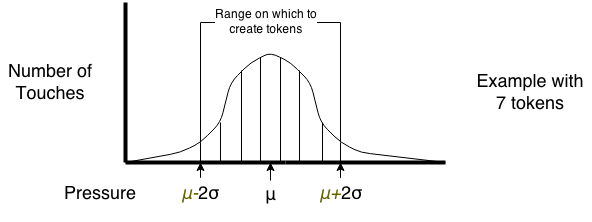
\includegraphics[width=3.6in]{token_creation.png}
\caption{Touch Tokens are Only Created for Pressure Values within Two Sigma Range for Each Key.}
\label{fig:token_creation}
\end{figure}


%TODO describe what is a Markov chain
Markov Chains are useful in predicting and modeling systems whose behavior evolves through discrete states. The probability of transitions between states can be captured.
In general an $n$-Markov model states that the
user tokens of length $n$ repeat themselves with certain frequency. Hence a user history
of $n$-token sequences could help us classify the user's future behavior. The tokens are
touch screen pressure values that are continually generated as the user interacts with an app
through a soft keyboard.

%Other information about Markov chains
%TODO traditional use of Markov chains
%Historically the Markov Chain has found applications in (statistics?)

%begin talking about the construction of the model
Instead of building a complete Markov model of the user behavior, we build a collection of $n$-grams
which are frequently instantiated sequences of $n$ tokens.
We use $n$-sized sequences  within a user interaction generated token sequence as an
$n$-gram which approximates $n$-Markov model. $n$-grams were originally
used in natural language processing \cite{Brown:ngram}.

%demonstrates how the range is split into many distinct token ranges by pressure

\begin{figure}
\centering
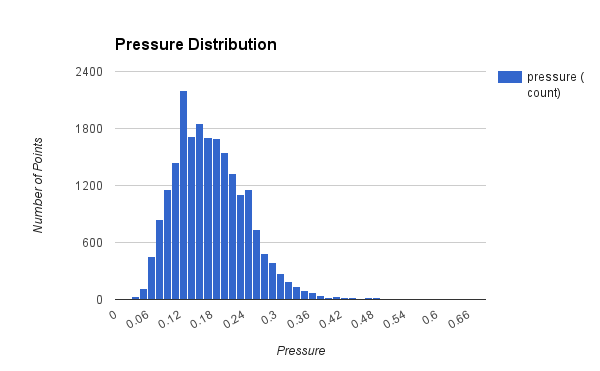
\includegraphics[width=3.6in]{normal_distribution.png}
\caption{This chart displays a set of pressure data from one of test users. Note that the pressure values are normally distributed.}
\label{fig:normal_distribution}
\end{figure}


%TODO continue talking about model construction.
%how are tokens constructed
%how are probabilities calculated
In building the model we remove some touches likely to be mistakes by the user or simply outliers in the data set.
The distribution of touch pressure values is calculated for each square button area on the touchscreen. 
In our system these areas correspond to keys of the soft keyboard. In order to develop PUF reproducibility,
the pressure tokens from the same key are 
assumed
%shown 
to have a normal distribution.
Figure \ref{fig:normal_distribution} plots a set of touch pressure values from one of the test users
%. which shows that this data is close to a normal distribution.

% show that our data is normally distributed
% useful resource: 
%   http://mathforum.org/library/drmath/view/72065.html
%\textbf{
%To verify pressure values generated by user on a given touch screen user are normally distributed,
%we preform the following statistical hypothesis test.
% TODO TODO TODO prove that pressure values are normally distributed
%}

From the token sequence, a normal distribution mean and variance ($\mu$ and $\sigma$) values are estimated for each soft keyboard key.
If a token pressure value falls outside of $\mu \pm 2*\sigma$ for a given key, 
then it is not included in any of the $n$-token sequences. 
Figure \ref{fig:token_creation} illustrates 
this tokenization process. The pressure values falling within $\mu \pm 2*\sigma$ are tokenized
into a predetermined $k$ tokens - 7 token ranges in Figure \ref{fig:token_creation}.
The value of $\mu\pm2\sigma$ was chosen because statistically $95.45$\% of touches 
will fall withing this range for normally distributed data \cite{threesigmarule}.
Tokens are compared both for the key (keyboard button) location and the tokenized pressure value.

%n-gram a continuious sequence of n items
%markov model for comparason is built from a sliding model of the previous n touches
%describe how the Markov chain is applied to touch pressure to model a user
%this is a description of our specific implementation of a Markov model
%\section{Touch Pressure Modeling}
%\label{touch_pressure_modeling}
% this section should describe various implementation details
%TODO it may be useful to include all different parameters to the model, and the effects of varying each of them

%describes how the Markov model is built from the sequence of touch pressures


%TODO desctibe, or reference somewhere, the above pictures

%TODO describe the Markov model used
Our goal in modeling user touch screen interactions with a Markov model is to classify the system in terms of its transitions between states. 
Each touch token contains information about the pressure and location of the interaction with the touchscreen.
These token fire off transitions.
In Figures \ref{fig:markov_model_building} and \ref{fig:final_markov_model_state}, 
Touch\_$n$ is a token and therefore comprised of a location and pressure range.
For instance, two user interactions with the same location
could be considered to be different touches in the model if
the they fall within a different range of pressure values.
In addition, two user interactions with different locations but with pressure
values within the same pressure range will be considered to be different touches.

\begin{figure}
\centering
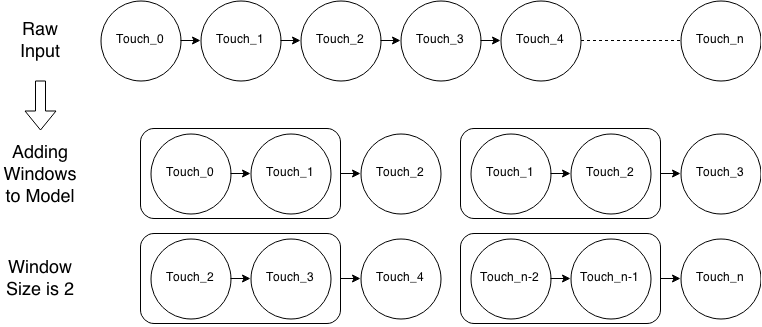
\includegraphics[width=3.4in]{figures/markov_model_building.png}
\caption{The top of this figure depicts the raw input touchscreen token sequence. Each touch represents a single interaction between the human user and the soft keyboard. The bottom part shows how the raw input is parsed into 2-Markov model. For example, the bottom left image can be interpreted to say that Touch\_4 succeeds the sequence Touch\_2, Touch\_3 with a non-zero probability.}
\label{fig:markov_model_building}
\end{figure}

%TODO describe aspects of the implementation
%describe how the model is constructed from the touch pressure sequence
Our Markov $n$-gram model calculates the probability of a given token following a specific 
token sequence of length $n$. Given a training sequence of tokens $T_0, T_1, \dots , T_N$,
we use maximum likelihood estimation (MLE) as follows to build the model. For all in-fixes of
length $n$: $T_i, T_{i+1}, \dots , T_{i+n-1}$, the following $n$-gram model is created:
$P(T | T_{i..(i+n-1)}) =  count(T, T_i, T_{i+1}, \dots , T_{i+n-1})/\sum_{T \in \Sigma} count(
T, T_i, T_{i+1}, \dots , \\T_{i+n-1}))$, where $T_{i..j}$ represents the
token sequence \\
$T_i, T_{i+\\1}, \dots, T_j$. Here, we are computing the probability of next token being $T$
given that the token sequence \\
$T_i, T_{i+1}, \dots , T_{i+n-1}$ has been seen. It is just the
frequency of this event in the token sequence $T_0, T_1, \dots , T_N$. \\
$count(T, T_i, T_{i+1}, \dots , T_{i+n-1})$ is given by the number of in-fixes with the same value as
$T_i, T_{i+1}, \dots , T_{i+n-1}$ followed by the token $T$. This gives 
$count(T, T_i, T_{i+1}, \dots , T_{i+n-1}) = \sum_{j=0}^{N-n}(1$ if $T_{j..(j+n-1)} == T_{i..(i+n-1)} \&\&
T_{j+n} == T)$.

Larger $n$ increases accuracy of the true probability of a given token $T$ following
a sequence $T_{i..(i+n-1)}$. The increased accuracy is due to the intuition that 
two users will be behave identically for  a sequence of $n$ tokens.
Figure~\ref{fig:markov_model_building} demonstrates how the token sequences for the Markov model are generated from the user's raw input from the soft keyboard.

%describes how the Markov model will look after it has been constructed
\begin{figure}
\centering
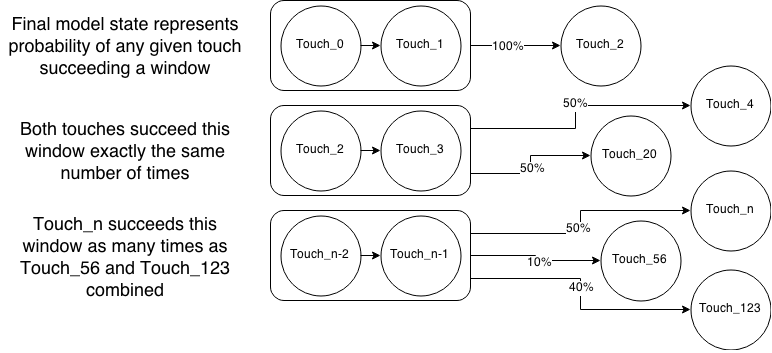
\includegraphics[width=3.4in]{figures/final_markov_model_state.png}
\caption{Example 2-Markov model after the probabilities have been calculated.
The rounded rectangles indicate that the touches inside are a window in the Markov model.
The top window states that Touch\_2 succeeds the sequence Touch\_0, Touch\_1 with probability 100\%.
Touch\_20, Touch\_56, and Touch\_123 are other touches which follow the preceding window with some probability.}
\label{fig:final_markov_model_state}
\end{figure}

%TODO describe the probability calculation in detail
Recall that the probability of a token $T$ following  a token sequence $T_{i..(i+n-1)}$ is 
expressed as the number of occurrences of $T$ succeeding the given sequence $T_{i..(i+n-1)}$ among
all the $N-n+1$ in-fixes of the sequence $T_{i..(i+n-1)}$.
The idea behind this probability calculation is illustrated in Figure \ref{fig:final_markov_model_state}.
Notably, Touch\_$n$ is not distinct. In other words Touch\_$a$ will be considered equal to Touch\_$b$ if the keycodes of these touches are equal and the touches fall within the same pressure range. Pressure ranges are depicted in Figure \ref{fig:token_creation}.

%TODO talk about how prefix tree is used to store these sequences in order to increase the speed.
%TODO cite some source which supports the benefits of a prefix tree
%TODO explain what a prefix tree is
%TODO include some figures to illustrate what a prefix tree is
The algorithm to calculate the $n$-gram probabilities of a token $T$ succeeding a given sequence
$T_{i..(i+n-1)}$ is the number of times that touch succeeds the sequence. This counts the  number of 
occurrences of $T_{i..(i+n-1)}||T$, where $||$ denotes concatenation.
The use of a prefix tree as a data structure helps keep track of appropriate
in-fixes and the affect of backtracking thus increasing the efficiency of this probability calculation.
%TODO explain how prefix tree makes them readily accessible

%TODO explain why this increases the speed of the probability caluclation... articulate how an alternative data structure would perform


%explain how the prefix tree is implemented in our system
In our system the $n$-token sequences are stored in a list while a prefix tree is used to store pointers to the instances of various tree prefixes in the list. 
The prefix tree nodes also include the count of number of occurrences of a sequence in addition
to a list of indexes/pointers to where the sequence occurs in the list storing all the sequences.
This index list is useful because it eliminates the need to search the list in order to determine what the successor tokens of a token window are.


%TODO this is the place for MLE, maximal liklihood estimation formulas


%basically the authentication scheme used
%frame it in more general terms, independent of our specific application
\section{Differentiating User-Device Pairs}
\label{sec:differentiation}
%TODO describe each of the model parameters in detail
%TODO state how each of the best model parameters were determined


%this figure describes how false positive and false negative percentages vary based on authentication threshold
\begin{figure}
\centering
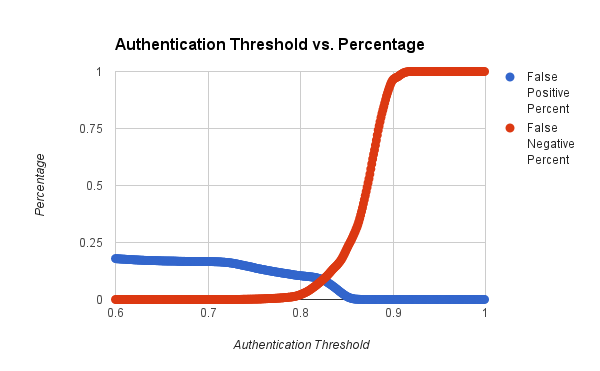
\includegraphics[width=3.6in]{threshold_vs_percentages.png}
\caption{False positive and false negative percentages vary as the authentication threshold is adjusted.}
\label{fig:threshold_vs_percentages}
\end{figure}

%TODO
%describe what the authentication threshold is
%define false positive
%define false negative
%explain why the intersection of these two is significant in choosing the authentication threshold
In distinguishing a user from another user, the $n$-grams for the two users need to be compared. 
For a given $n$-gram $[(T_{i_0} T_{i_1} \dots T_{i_{n-1}}), (p_0, p_1, \dots, p_k)]$ where 
$(T_{i_0} T_{i_1} \dots T_{i_{n-1}})$ is the prefix sequence and $(p_0, p_1, \dots, p_k)$ is the
probability vector for the next token being Token 0, Token 1, ..., Token $k$ from the alphabet $\Sigma$.
The distance between two $n$-grams $distance[(T_{i_0} T_{i_1} \dots T_{i_{n-1}}), (p_0, p_1, \dots, p_k)]$
and \\
$[(T_{i_0} T_{i_1} \dots T_{i_{n-1}}), (q_0, q_1, \dots, q_k)]$ is
given by \\
$\Sigma_{j=0}^k|(p_j - q_j)|/(k+1)$ where $|x|$ is the absolute value of $x$.
The difference between two user profiles is the average difference between $n$-grams belonging
to the two profiles. If the two $n$-grams are identical, the distance is 0.
One minus this distance is a measure of the {\it divergence} between two user profiles.

Continuous authentication system needs to determine when two sets of touch pressure values came from the same user-device pair. When authenticating a user, we take the difference between
the user profile $n$-grams constructed from the training data set and the $n$-grams
constructed from the current touch interaction data. The confidence interval
that the current user is the same whose training profile exists can be given $1 - 
avgDistance(TrainingProfile \; n-grams, \; CurrentProfile \; n-grams)$. If the two profiles are
identical with distance 0, confidence level in the user identity is highest at 1.
%
%add more metrics, and explain them, provide more graphs about them
If authentication is a binary decision of yes or no, a threshold value $0 \leq th \leq 1$ is set.
if the ConfidenceInterval $= 1 -$ ProfileDistance $> th$, the user is authenticated; otherwise not. 
Figure \ref{fig:threshold_vs_percentages} illustrates how false positive percentage and false negative percentage rates vary based on the threshold value for authentication. 

%authentication threshold described

%false positive percentage described
False positive rate measures the fraction of authentications between two touch token profiles where 
the two profiles did not come from the same user-device pair.
False negative rate is exactly the inverse of false positive rate in that it describes the
frequency with which the two touch token profiles from the same (user, device) pair fails the authentication. 

%significance of the intersection of false positive, false negative values
In Figure \ref{fig:threshold_vs_percentages} there exists a clear intersection between false negative and false positive percentages. This intersection is significant; at this point the system is not biased towards
either of false positive or false negative events. This point represents a balance in design. For our
data sets, this balance point was approximately at $th=0.83$. For a threshold in the range
$0.6 \leq th \leq 0.83$, false negative rate was close to 0 at the cost of a false positive rate approaching 0.2.
The choice of this threshold will depend on the authentication requirements.

% this figure describes the effect of window size on authentication accuracy
\begin{figure}
\centering
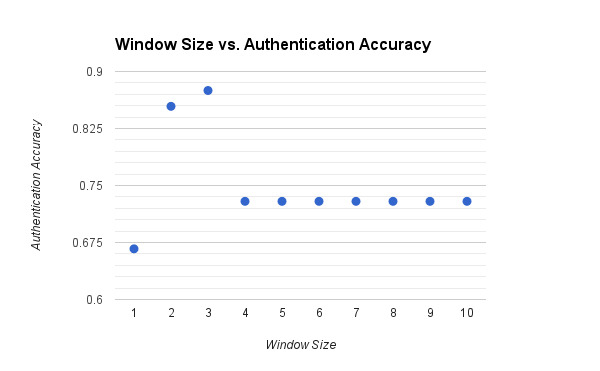
\includegraphics[width=3.6in]{window_size_vs_authentication_accuracy.png}
\caption{The effect of $n$ in $n$-Markov Model window size on authentication accuracy.}
\label{fig:window_size_vs_authentication_accuracy}
\end{figure}

%TODO describe the effect of window size on authentication accuracy
The link between model parameter window size and authentication accuracy is demonstrated by Figure \ref{fig:window_size_vs_authentication_accuracy}.
The window size parameter is equivalent to the $n$-gram size in our $n$-Markov Model.
The results in this chart were generated by holding all other model parameters constant and varying the window size. This approach was chosen to isolate the effects on authentication accuracy resulting from window size.
Window size achieves the greatest authentication accuracy at a size of $n=3$ with the authentication threshold set to $th=.75$.
Varying the authentication threshold to $th=0.9$, authentication accuracy reaches its maximum at $n=2$. 
The authentication threshold can be set at $th=0.5$ to achieve a result of $n=4$ providing maximum authentication accuracy.
From this we conclude that $n={2,3,4}$ to be viable options for this model parameter.


\section{Data Collection and Analysis}
\label{sec:data_collection}
%TODO
%describe the number of users from which the data was collected
%describe the method of collection
Data for touch pressure models in this experiment was generated using a special keyboard application for the android operating system. Users would load the keyboard onto their device and continue using the device in the way they normally would. Some users were asked to play a typing game in order to help expedite the data collection process. After the users had generated at least ten thousand touches the data was collected from the user's device to train the profile.
%TODO put the data in context by detailing the number of touches collected from each user and the number of touches used to build the model

%TODO describe the user base from which the data was collected for the results presented here
The results presented here were derived from the touch data generated by two users. These users each used two different devices creating four user-device pairs each having a large number of touches.

%TODO describe how the data was analyzed


%what number of states exposed the most uniqueness e.g. how many tokens were best
%with what accuracy could users be distinguished from one-another
\section{Results}
\label{sec:results}
%TODO discuss predictions and whether they were correct or incorrect.

%this section describes how authentication accuracy was investigated. Also included are a few figures which describe the best authentication accuracy percentage
\begin{figure}
\centering
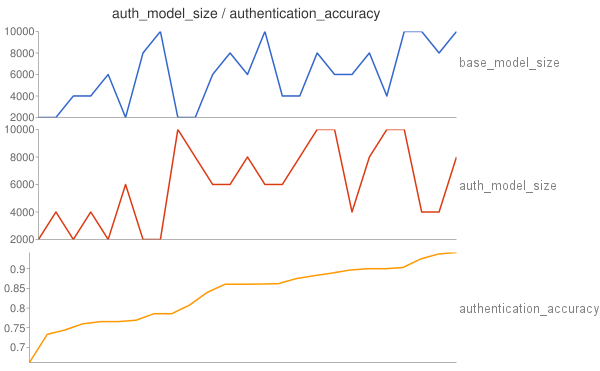
\includegraphics[width=3.5in]{authentication_accuracy_vs_model_size.png}
\caption{Authentication accuracy is a function of
both the base model size and authentication model size.
This graph is aligned on the horizontal axis.}
\label{fig:authentication_accuracy}
\end{figure}

%explain the contents of this figure.
%explain what each of the metrics used in the figure are.
%
The two key parameters left to determine are the training data set size (base model) and the 
authentication data set size (authentication model). The figure of merit is authentication accuracy.
Figure \ref{fig:authentication_accuracy} shows {\it authentication\_accuracy} as a function of {\it base\_model\_size} 
and {\it auth\_model\_size}. We define {\it authentication\_accuracy} to be the percentage of authentications for which our system makes the correct decision (both false positives and
false negatives count against the accuracy).
In other words, an authentic user is authenticated and a non-authentic user is not authenticated.
The size of base model and user model which result in a given authentication accuracy are aligned with that authentication accuracy on the horizontal axis in the chart.
An example data point
might be read as follows: base\_model\_size of
6000 touches and auth\_model\_size of 6000 touches
results in 85\% authentication accuracy.

%explain why more touches does not always equal more accuracy
Both the base model and the authentication model sizes were varied between 2000-10,000 touches.
In some instances, increased numbers of touches did not result in higher authentication accuracies. 
Part of this has to do with the way the distance between the base model and the authentication
model is computed. Existence of an $n$-gram in authentication model that does not belong to the base model
is considered an unlikely event, and hence an anomaly. It is penalized in the distance computation
by computing absolute distance as its probability $Prob(NG[i, auth])$ - probability of an $n$-gram
$i$ in the base model. Hence if this probability is $.75$, its contribution to
confidence interval is only $1-0.75=0.25$.
An authentication model whose size exceeds the base model size by a significant margin usually
does not benefit the authentication accuracy. The authentication model includes some
$n$-gram sequences that were not seen in the training base model. Hence, they do not add much to the
authentication accuracy.

A small sized base model suffers in the authentication accuracy for the same reasons. 
The number of $n$-grams is low in the base model.  Then the difference value between the base
model and the authentication model will be high due to the penalty assessed on the authentication model
$n$-grams that do not exist in the base model. 

%describes authentication accuracy dependence on the amount of user data
\begin{figure}
\centering
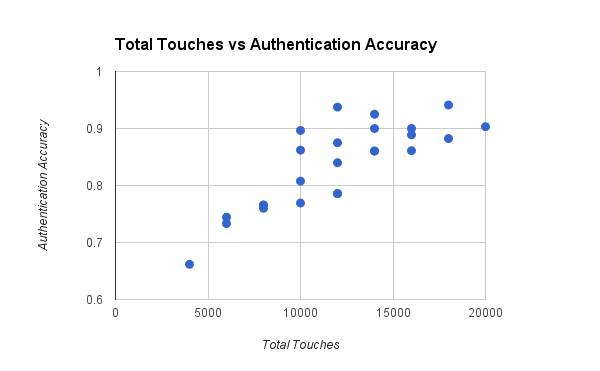
\includegraphics[width=3.5in]{total_touches_vs_authentication_accuracy.png}
\caption{Authentication accuracy is linked more closely to the total number of touches used in the authentication then to either the base model size or the authentication model size. Although authentication accuracy does not strictly increase with the number of touches it does trend upward.}
\label{fig:total_touches_vs_authentication_accuracy}
\end{figure}

%TODO explain the contents of this figure.
%explain what each of the metrics used in the figure are.
%
Figure \ref{fig:total_touches_vs_authentication_accuracy} presents the tradeoff between the amount of data needed for an authentication and the accuracy of that authentication.
In general, more data will yield a better authentication accuracy, but this is not always true.
The size of the base model seems to contribute more to authentication accuracy then does the size of the authentication model, therefore, if the goal is to increase authentication accuracy it is better to increase the size of the base model compared to increasing the size of the authentication model.


%TODO remove, and remove all reference to this
%\begin{figure}
%\centering
%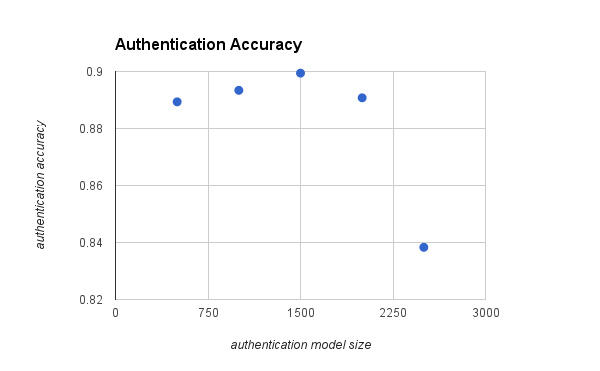
\includegraphics[width=3.9in]{extensive_authentication_accuracy.png}
%\caption{Depicts the result of many model comparisons done around the area of best results in Figure \ref{fig:authentication_accuracy}.}
%\label{fig:extensive_authentication_accuracy}
%\end{figure}

%explain the contents of this figure.
%explain what each of the metrics used in the figure are.
%
%To establish that the results in Figure \ref{fig:authentication_accuracy} hold for large numbers of comparisons many more comparisons where done around the area of best results. The results of these tests are presented in Figure \ref{fig:authentication:accuracy}. For the results depicted in the figure, user\_model\_size is held constant at ten thousand while auth\_model\_size is varied. The test was performed in this way because variations in auth\_model\_size seems to have a greater impact on authentication accuracy than variations in base\_model\_size. Approximately the same trend as seen in Figure \ref{fig:authentication_accuracy} presents itself in Figure \ref{fig:extensive_authentication_accuracy}.

%explain the contents of these figures.
%explain what each of the metrics used in the figure are.
%fig:nexus_speed_test
Figure \ref{fig:nexus_speed_test} displays the execution time of our system on a Nexus 7 tablet. Time taken is measured in milliseconds while model sizes are measured by number of touches used to construct the model. 
The time metric does not include the overhead associated with adding touches to either the base or auth models. It is assumed this will be done over time as the user enters data. In addition, adding touches is not a computationally intensive activity - more of a UI event. 
Time does include the probability computation for each of the models and the comparison between the models.
This chart is a good representation of how each of the model sizes affects the execution time of the system.
 The overall time taken is trending upward linearly in the total base model size and auth model size.
 This suggests that the total number of touches used, that is the sum of base model size and auth model size, dictates the authorization efficiency.
The time dependence on the total number of touches makes sense because the  probability computations in
Markov model dominate. 
Also of note, the base model size and auth model size seem to affect time taken differently. A change of 
factor $k$ in the size of auth model seems to increase the total amount of time taken more than the same $k$-sized change in the base model. 

\begin{figure}
\centering
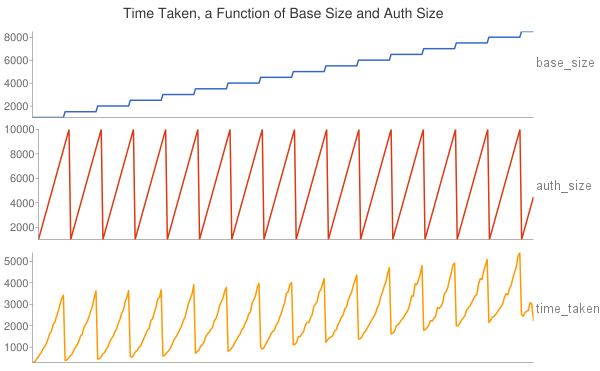
\includegraphics[width=3.5in]{nexus_speed_test.png}
\caption{The authentication time on a Nexus 7 tablet as a function of base model size and auth model size. Time taken is measured in milliseconds while model sizes are measured by number of touches.}
\label{fig:nexus_speed_test}
\end{figure}

%fig:nexus_total_size_time
Figure \ref{fig:nexus_total_size_time} illustrates how the execution time depends on the total number of touches used in creating the models. The trend suggests that the total  time  increases 
nonlinearly as the number of touches used to generate the model increases.
This figure also supports the conclusion that the total size of the model in number of touches has a larger influence on the execution time then the sizes of either the base or auth models individually.
This graph is aligned on
the horizontal x-axis. As an example, a data point
might be read as follows: base\_size of 6000
touches and auth\_size of 10000 touches results in
4000 millisecond run time on a Nexus 7 tablet.

\begin{figure}
\centering
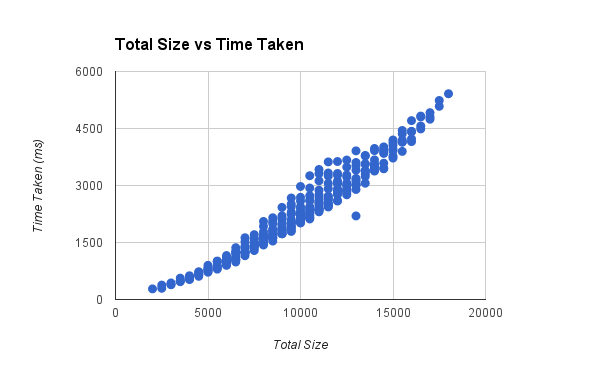
\includegraphics[width=3.5in]{nexus_total_size_time.png}
\caption{The execution time  on a Nexus 7 tablet as a function of base model size plus auth model size.
Time taken is measured in milliseconds while model sizes are measured by number of touches.
This graph is aligned on the horizontal axis.}
\label{fig:nexus_total_size_time}
\end{figure}

The execution time  increases
with the number of touches used in the Markov model.
For a targeted accuracy, as Figure \ref{fig:total_touches_vs_authentication_accuracy} observes, a certain minimum
number of touches are needed in the model.
This presents a problem if the execution time
resulting from this minimum bound on the
number of touches in the model is high. Our
tests  on the Nexus 7 tablet show the execution time
stays below 6 seconds
with the  total number of touches in the model bounded by 18000.
Figure \ref{fig:nexus_total_size_time} shows this trade-off between number of touches
in the model and the corresponding execution time.

%TODO discuss why each figure is important
%figure x establishes that x model size has a greater influence on the speed and that overall performance seems to be in some way a function of the total number of touches used.
%figure x2 establishes that there is an exponential trend in the runtime of this system. As 

%tie it all together, discuss the importance of this section as a whole
Figures \ref{fig:authentication_accuracy}  \& \ref{fig:total_touches_vs_authentication_accuracy} establish that in general a greater number of touches used in the authentication will result in a greater accuracy. This manifests in the charts as the peaks of highest authentication accuracy  
corresponding to the largest numbers of touches. Figures \ref{fig:nexus_speed_test} and \ref{fig:nexus_total_size_time} demonstrate the performance tradeoff associated with increased numbers of touches. 
As expected there exists an inverse relationship between performance in terms of speed and accuracy of authentication. That is, increased authentication accuracy comes at the expense of execution time. 

\section{Distributed User-Device (UD-) PUF}
\label{sec:PUF}
The preceding discussion extends the human-device entangled PUFs \cite{ScheelTyagi15} to a distributed
implementation. The $n$-Markov model also determines frequently occurring $n$-token sequences for a
given user. All of these $n$-token sequences can be considered to be the challenge set. The resulting
pressure value responses can then be quantized into a binary response in the same way as in 
\cite{ScheelTyagi15} resulting in the same variability and reproducibility properties. The main 
difference is that this distributed PUF is derived as a side-effect of the authentication mechanism.
This could support alternate functionalities that can benefit from a PUF based on the user-device 
physical randomness.

\section{Conclusions}
\label{sec:conclusions}
%make sure to re-tell the story in the conclusion.
%describe what has been presented in the paper
This paper presents a continuous authentication approach which utilizes the variability in the way users interact with the touchscreens of their devices to differentiate distinct user-device combinations. 
A continuous authentication model prevents data theft from a mobile device even for lost devices.

Our experiments establish optimal training data set sizes around 6000-10000 touches, an authentication
data set size at around 4000 touches, and the $n$-gram sequence length in the range 2-4. This leads to
authentication accuracy over 80\% with both false positive and false negative rates contained
below 12\%.
%describe the implementation, model, authentication
%TODO discuss the advantages to using an n-Markov model over other modeling systsms


%TODO possible, describe applications  in terms of continuous authentication

%\bibliographystyle{abbrv}
\bibliographystyle{unsrt}
\bibliography{bibliography/markov_chains,bibliography/pufs,bibliography/other,pufs}

% Ignore incorrect citation numbering
%\ignorecitefornumbering
%\bibliographystyle{unsrtnat}

\end{document}
